\begin{figure}[H]
\centering
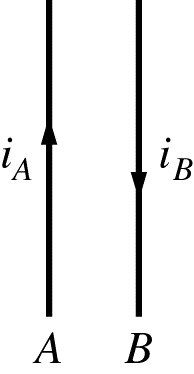
\includegraphics[scale=0.3]{images/img-012-037.png}
\end{figure}

% Multiple Choice Question 28
\begin{questions}\setcounter{question}{27}\question
Two parallel wires, $A$ and $B$, have currents in opposite directions, as shown in the figure above. Current $i_{B}$ is twice as large as $i_{A}$. The force on wire $A$ due to current $i_{B}$ has magnitude $F$. Which of the following correctly describes the direction and magnitude of the force on wire $B$ due to current $i_{A}$?

\tabto{0.75cm}\underline{Direction}
\tabto{4.00cm}\underline{Magnitude}

\begin{choices}
\choice To the left  \tabto{3.25cm} $F$
\choice To the left  \tabto{3.25cm} $2 F$
\choice To the left  \tabto{3.25cm} $4 F$
\choice To the right \tabto{3.25cm} $F$
\choice To the right \tabto{3.25cm} $2 F$
\end{choices}\end{questions}

